\documentclass[11pt,a4paper]{article}
\usepackage[utf8]{inputenc}
\usepackage[T1]{fontenc}
\usepackage{amsmath,amsfonts,amssymb}
\usepackage{apacite}
\usepackage{natbib}
\usepackage{graphicx}
\usepackage{booktabs}
\usepackage{threeparttable}
\usepackage{array}
\usepackage{url}
\usepackage{hyperref}
\usepackage[margin=2.5cm]{geometry}
\usepackage{setspace}
\usepackage{comment}
\usepackage{outlines}
\onehalfspacing

\newcommand{\Var}{\text{Var}}
\newcommand{\Cov}{\text{Cov}}

% Define \sym command for significance stars from esttab
\newcommand{\sym}[1]{{#1}}

\title{Debiasing Second Moments of Estimated CEO Effects: A Placebo-Controlled Approach\thanks{Project no. 144193 has been implemented with the support provided by the Ministry of Culture and Innovation of Hungary from the National Research, Development and Innovation Fund, financed under the KKP\_22 funding scheme. This project was funded by the European Research Council (ERC Advanced Grant agreement number 101097789). Telegdy received support from the Hungarian Scientific Research Fund – OTKA, contract number 143346. The views expressed in this research are those of the authors and do not necessarily reflect the official view of the European Union or the European Research Council.}}

\author{Miklós Koren\thanks{Central European University, ELTE Centre for Economic and Regional Studies, CEPR and CESifo. E-mail: korenm@ceu.edu} \\
        Krisztina Orbán\thanks{Monash University.} \\
        Álmos Telegdy\thanks{Corvinus University of Budapest. E-mail: almos.telegdy@uni-corvinus.hu}}

\date{October 2025}

\begin{document}

\maketitle
\thispagestyle{empty}

\begin{abstract}
Understanding the link between estimated manager effects and firm outcomes is central to research on CEOs and firm performance. While firm and CEO fixed-effect estimators of mean CEO effects are unbiased under random mobility, most applied analyses use second moments of these estimates — variances, covariances, correlations, and event-study dynamics — that are systematically biased by small-sample noise. We develop a placebo-controlled event-study design that identifies and removes these biases without modeling the full error process. The method constructs placebo transitions that replicate the spell-length design of actual transitions while excluding periods around real changes. Moments computed on placebo spells recover the bias components that inflate variances and covariances; subtracting them yields debiased moments and regression slopes. A Monte Carlo study with six scenarios — baseline, long panel, persistent errors, unbalanced panels, excess variance, and all complications — illustrates when the correction matters most. We outline an application to the universe of Hungarian firms (1992--2022) that examines pre-trends and dynamic effects after CEO arrival, a common use case in the literature.
\end{abstract}

\textbf{Keywords:} CEO value, CEO-Firm Fixed Effects, Bias Correction

\textbf{JEL Classification:} C23, D24, G34

\clearpage
\setcounter{page}{1}

%%%%%%%%%%%%%%%%%%%%%%
\section{Introduction}
%%%%%%%%%%%%%%%%%%%%%%

The impact of individual CEOs on business practices and firm performance is a widely studied question in economics, corporate finance, and management. In absence of direct measures of CEO characteristics relevant for firm outcomes, studies often include CEO fixed effects to capture variations in latent CEO skills. [[cite Bertrand Schoar, more econ papers, also Strategic Management journals]] Under the standard assumption of ``random mobility,'' that is, CEO moves are unrelated to past and future performance shocks of the firm, the mean of estimated CEO fixed effects is unbiased \citep{}. 

Most applied work, however, is concerned with the second moments of the estimated fixed effects. First, variance decompositions reveal how much CEO effects contribute to the variance of certain firm outcomes, such as productivity or profitability \citep{}. Second, to understand the mechanisms through which CEOs affect firm outcomes, the estimated CEO effect is often used to assess its effect on other variables which is based on the covariance. For example, whether firms led by better CEOs are more profitable \citep{mackey2008effect} or how much risk they take \cite{schoar2024effect}. Third, dynamic covariances are used in event studies to assess how outcomes evolve before and after CEO transitions, as a way to test for pre-trends and to understand post-transition dynamics \citep{schoar2024effect}.

All these second moments are biased by small-sample noise in the estimated CEO effects, even under credible identification assumptions \citep{andrews2008high,gaure2014correlation,Bonhomme2023-dx}. This is not a nuisance, but has important implications for the interpretation of empirical results. Perhaps most intuitively, small-sample bias overstates the role of CEOs in explaining firm performance. [[FIXME: ise a good outcome variable to explain the second bias]] And, as we show below, the bias introduces spurious pre-trends and distorts post-transition dynamics in event studies.

Correcting for small-sample bias is challenging. Existing methods are either ad hoc, such as leave-one-out adjustments with the goal of removing own-observation noise \citep{}, or highly structural: estimate the bias from the variance-covariance of shocks and the design matrix and then apply Empirical Bayes shrinkage \citep{andrews2008high,Bonhomme2023-dx,kline2024firm}. While powerful, these require estimating many components and re-deriving formulas for each target second moment.

Our approach is different: we create a placebo-controlled experiment. For each firm that truly changes CEOs, we find a group of comparable non-changing firms, and use this placebo control group to estimate the mechanical noise in the second moments.\footnote{This step in the spirit of \cite{jarosiewicz2023revisiting}, who compare the replicated results of \cite{Bertrand2003-io} with placebo regressions.} Under weak assumptions, the placebo group can be used to measure the exact bias in variance, covariance, and dynamic covariance. The difference in second moments between the treated and the placebo groups yields debiased estimates, without having to model and estimate the full variance-covariance structure of errors.

We illustrate our method in Monte Carlo experiments. [[EXPLAIN]]

We then use our method to measure the quantitative contribution of CEOs to firm growth in Hungarian data, 1992-2022. [[EXPLAIN]]

Our method relies on two key assumptions about the nature of shocks. First, we assume strict exogeneity, that is, error terms are mean independent of the CEO path for all time periods. This ensures that the estimated CEO effects are mean unbiased. Second, we assume that the autocovariance of errors is the same between treated and control firms, up to a scalar multiplier. In other words, we allow for treated firms to be more volatile than control firms, but we assume that the temporal correlation structure of shocks is unchanged. We call this assumption ``parallel second moments,'' in reference to the weaker parallel trends assumption in difference-in-differences designs. Other than these two assumptions, we make no further restrictions on the error process, the number and length of CEO spells, or the heterogeneity of CEO effects.

To understand how these assumptions help debias the variance-covariance of estimated CEO effects, note that the bias terms are weighted sums of the autocovariances of errors, with weights depending on the research design, including the spell length of CEOs at each firm. The placebo design ensures that treated firms and control firms have the same spell-length distributions, and therefore the same weights. The parallel second moments assumption then implies that the bias terms are the same up to a scalar. And because covariance is a bilinear operator and variance is additive under strict exogeneity, the bias terms can be ``precomputed'' in the placebo group and simply subtracted from the treated moments.\footnote{This is not true for nonlinear transformations of variances and covariances, such as correlations and regression slopes. In these cases, we first debias all underlying variances and covariances and only then form the ratio.} In summary, the placebo group, by construction, has no CEO effects, so the variance and covariance of estimated placebo effects identify the bias terms. Subtracting these from the treated moments yields debiased estimates.

XXX

The main idea of this correction is the creation of pseudo CEO transitions in the data. We take firms with CEO transitions, record their event window. The event window is the period encompassing the years under the CEO prior to the CEO change and the period under the new CEO post the change. We match these firms to firms born in the same year, belonging to the same sector, that however do not experience a CEO transition during the years of the event window. Then, we assign to the control firms a placebo CEO transition happening in the same year as the treated firm experiences the true CEO transition.\footnote{In addition to addressing the limited mobility bias, our approach has the advantage of creating a control group that is more similar to the treated firms than the universe of firms}. On the matched sample we implement two-way fixed effects regressions.\footnote{The estimation is similar to the two way fixed effects regression developed by \cite{Callaway2021JoLE}, but we exploit the fact that the control group also has a time of pseudo CEO change. We compare firms with a true CEO change with firms with a fake CEO change along the same event-time years.} If estimated `effects' for these pseudo-CEOs diverge substantially, this reveals the noise problem in fixed effects estimation. By comparing actual CEO transitions to these placebo transitions, we can correct the fixed effects estimates for noise, isolating the true CEO contribution.

%Why is our approach unique - data
Papers use three approaches when analyzing the effect of CEOs. One group studied the effects of a distinct, measurable variable, such as managerial practices used in the firm \citep{bloom2012organization} or a CEO attribute (age, gender, tenure, education or country of origin \citep{anderson2018pathways, henderson2006quickly, Koren2023expat}). These studies are useful to show the effects of the studied variables, but they arguably capture little of the whole effect of CEOs over the firms they manage. Another group uses an external event to assess the effect of CEO turnover (e.g., \citet{bennedsen2020ceos}). While this approach brought about credible causal estimates, the heavy data needs render this approach impossible to use in most situations. 

The third group employed firm and CEO fixed effects to separate the quality of firm from that of the CEOs \citep{Bertrand2003-io, crossland2011differences, quigley2015has}. While these studies employ a framework that can be used in many settings, the generalizability of their results is challenged by the data used because almost all study public companies only.\footnote{\citet{quigley2022ceo} is a notable exception studying CEO effects in private businesses, but the private sample comprises of large firms.} Our data has information on the universe of Hungarian businesses and all their CEOs for the period between 1992 and 2022, tracking over 1 million firms and a similar number of CEOs.\footnote{Mandatory registration of all company directors ensures complete coverage of CEOs in the whole corporate sector.} The overwhelming majority of the firms in our sample are small and medium-sized enterprises (SMEs). This adds a new dimension to the analysis that was largely missing from the literature and allows drawing conclusions about CEOs' effects on the whole economy. Our analysis is also distinctive in that earlier studies focused on developed countries, while our data come from Hungary. Indeed, the institutional context matters: \citet{crossland2011differences} show that informal and formal institutions affect CEO discretion.

To quantify the effect of CEOs on firm performance in our data, we perform a variance decomposition, which computes what proportion of the total dispersion of productivity change is explained by CEO transitions. As demonstrated by countless papers in labor economics, the variance is also contaminated by the limited mobility bias and we make a correction of it with the  placebo method. With our carefully chosen control group we also take into account the mechanical effect of firm age on productivity dispersion: as time passes, the firm gathers shocks and so the dispersion will increase. 

We find that CEO transitions explain about 30\% of the productivity change in our data. The placebo correction is also important here: without it, this share would be about twice as large.

%literature
Our work connects to the broader literature on management practices and firm productivity. Randomized controlled trials demonstrate that management training and consulting improve firm performance \citep{bloom2013does, mckenzie2021small}, but these interventions change practices rather than people. Whether replacing managers generates similar gains remains contentious. Evidence from public sector organizations suggests modest manager effects \citep{fenizia2022managers, janke2024role}, while studies of family firms find larger impacts when professional managers replace family members \citep{bennedsen2007inside, sraer2007performance}. Our results for private firms fall between these extremes: CEOs matter, but less than raw correlations suggest.

Methodologically, our paper builds on the two-way fixed effects literature in labor economics that decomposes wages into worker and firm components \citep{Abowd1999Econometrica, Card2018JoLE}. These studies face similar challenges from limited mobility creating small-sample bias \citep{andrews2008high} and have developed bias-correction methods \citep{Bonhomme2023-dx, gaure2014correlation}. We adapt this framework to the CEO-firm setting but add placebo controls to separate signal from noise. This approach is valuable when studying managers who, unlike workers, have few observations per individual, making traditional bias-correction methods less effective. Recent work has documented apparently increasing CEO effects over time \citep{quigley2015has}, but these studies do not account for the mechanical noise we identify. \citet{lippi2014corporate} find that concentrated ownership in Italian firms distorts executive selection and reduces productivity by 10\%, providing motivation for our framework separating owner and CEO decisions.

%%%%%%%%%%%%%%%%%%%%
\section{The Econometric Problem}
%%%%%%%%%%%%%%%%%%%%

Let firm $i$ in year $t$ have outcome
\begin{equation}\label{eq:model1}
  y_{it} = z_{m(i,t)} + e_{it},\qquad \mathbb E[e_{it}|z_{is}]=0,
\end{equation}
where $z_{m(i,t)}$ collects the CEO effect at time $t$ and $e_{it}$ is a shock. We assume that $z_{m(i,t)}$ is piecewise constant, changing only when the CEO changes and that $e_{it}$ is mean independent of the CEO path for all $s$ (``strict exogeneity'' or ``random mobility'').

Under the strict exogeneity assumption, the ordinary least squares (OLS) estimator of $z_m$ is unbiased. Equation \eqref{eq:model1} can be rewritten as a dummy-variable regression 
$$
y_{it} = \sum_{n} z_n D_{m(i,t)=n}  + e_{it},
$$
and the first-order condition for the OLS estimator $\hat z_n$ is
$$
0 = \sum_{i,t:m(i,t)=n} (y_{it} - \hat z_n),
$$
or 
$$
\hat z_n = \frac{1}{T_n} \sum_{i,t:m(i,t)=n} y_{it} = z_n + \frac{1}{T_n} \sum_{i,t:m(i,t)=n} e_{it},
$$
where $T_n$ is the number of observations with CEO $n$. The estimator is unbiased because $\mathbb E[\hat z_n|z_n] = z_n$. The estimator, however, is only consistent as $T_n\to\infty$, that is, as the number of observations per CEO grows large. In practice, many CEOs have short tenures, so $\hat z_n$ contains substantial noise.\footnote{The mean CEO tenure (standard deviation) is 13.8 (1.7) in US small and medium-sized companies \citep{simsek2007ceo}, 8.1 (5.8) in US public companies \citep{brookman2009ceo}. The large standard deviations demonstrate that many CEOs have only a few years long tenure.} 

Econometric applications often require the second moments of $\hat z_n$, for example, to estimate the variance of CEO effects or to run regressions of an outcome $y_{it}$ [[this is another outcome than in eq (1), right?]] on $\hat z_n$. The former could inform us about the importance of CEO heterogeneity (REFs), while the latter about the effect of CEO quality on firm performance and firm policies (REFs). 

The small-sample error, however, contaminates \emph{all second moments} of $\hat z_n$. The variance of $\hat z_n$ is inflated relative to the variance of true CEO effects $z_n$ (REFs), and the covariance of $\hat z_n$ with other variables that are affected by $e_{it}$ is also contaminated. A well-known example of this in the labor literature is ``limited mobility bias'' \citep{andrews2008high}, which states that in a two-way fixed effects model of worker and firm effects, the variance of both effects is biased upwards, and their correlation is biased downwards.

Existing methods of bias correction for second moments take two broad forms. One is ad hoc, such as leave-one-out adjustments that hope to remove own-observation noise \citep{kline2020leave} [[I would not call it ad hoc, they derive that the variance is unbiased]]. These can be impractical in CEO settings with a single manager per firm-year and lack formal guarantees. The other is structural: estimate the bias from the variance–covariance of shocks and the design matrix and then apply Empirical Bayes–type shrinkage (e.g., \citealt{andrews2008high}, \citealt{Bonhomme2023-dx}). While powerful, this requires estimating many components and re-deriving formulas for each target second moment. Our approach is different: we construct placebo transitions that replicate the treated design matrix and use the placebo moments to read off the bias term directly, then subtract it. This delivers debiased variances, covariances, and slopes without modeling the full shock process.


\newenvironment{example}{\par\noindent\textbf{Example.}\ }{\par}

To fix ideas, consider the following example. While our method is more general, the example captures its key elements.
\begin{example}
Event window $t\in\{-2,-1,0,+1,+2\}$ with baseline $t=-1$. Pre-spell length $T_1=2$ (years $-2,-1$ under CEO A). Post-spell length $T_2=3$ (years $0, +1,+2$ under CEO B). The contrast of interest is the change from the baseline year $t=-1$ to three years after the transition $t=+3$:
\[
y_{i,+3} - y_{i,-1}.
\]
\end{example}

Stack outcomes as $\mathbf y_i=[y_{i,-2},\,y_{i,-1},\,y_{i,0},\,y_{i,+1},\,y_{i,+2}]'$. Define the piecewise-constant CEO path $\mathbf z_i$ so that $z_{i,-2}=z_{i,-1}$ (CEO A), $z_{i,0} = z_{i,+1}=z_{i,+2}$ (CEO B). The linear contrast for the example is implemented by the weight vector
\[
  \mathbf w = [\,0,\,-1,\,0,\,0,\,+1\,]',
\]
so that 
$$
y_{i,+3} - y_{i,-1} = \mathbf w' \mathbf y_i.
$$

\paragraph{Model setup.} We are now ready to present the general setup in matrix notation. Let firm $i$ be observed for $T$ periods with outcome path $\mathbf y_i\in\mathbb R^T$ that decomposes into a (piecewise-constant) manager-effect path $\mathbf z_i$ and shocks $\mathbf e_i$. Suppose manager 1 serves in the first $T_1$ periods and manager 2 in the last $T_2=T-T_1$ periods. (Other transition paths can be modeled similarly.) The model is
\begin{equation}
\mathbf y_i = \mathbf z_i + \mathbf e_i
\end{equation}
with 
\begin{equation}
\mathbb E[\mathbf z_i\mathbf z_i']= \mathbf \Lambda_i=
\begin{bmatrix}
  \lambda_{i11}\otimes \mathbf{11}' & \lambda_{i12}\otimes \mathbf{11}'\\
  \lambda_{i12}\otimes \mathbf{11}' & \lambda_{i22}\otimes \mathbf{11}'
\end{bmatrix},
\qquad \mathbb E[\mathbf z_i\mathbf e_i']=0,
\qquad \mathbb E[\mathbf e_i\mathbf e_i']=\sigma_1\mathbf\Sigma
\end{equation}
for changing firms, and 
\begin{equation}
\mathbb E[\mathbf z_i\mathbf z_i']= \mathbf \Lambda_i=
  \lambda_{i11}\otimes \mathbf{11}',
\qquad \mathbb E[\mathbf z_i\mathbf e_i']=0,
\qquad \mathbb E[\mathbf e_i\mathbf e_i']=\sigma_0\mathbf\Sigma
\end{equation}
for non-changing firms. The first equation is just notation for the variance and covariance of manager fixed effects at firm $i$. These are the objects of interest. The second equation states the standard strict exogeneity assumption, often called ``random mobility'' in such designs. Every period's shock is mean independent of the entire CEO path. The third assumption allows for arbitrary autocorrelation in shocks over time (e.g., persistent shocks), but assumes that this autocorrelation is the same for changing and non-changing firms, up to a scalar multiplier $\sigma_1/\sigma_0$. We call this assumption ``parallel second moments,'' in reference to the weaker parallel trends assumption in difference-in-differences designs.

For any linear contrast with weights $\mathbf w\in\mathbb R^T$ and $\mathbf w'\mathbf 1=0$, define $\Delta y_i=\mathbf w'\mathbf y_i$, $\Delta z_i=\mathbf w'\mathbf z_i$, and $\varepsilon_i=\mathbf w'\mathbf e_i$, resulting in
\begin{equation}\label{eq:contrast}
\Delta y_i = \Delta z_i + \varepsilon_i.
\end{equation}
The weight vector may be computing first differences, long-run differences relative to a baseline, or an average of pre- and post-periods of CEO arrival. We require $\mathbf w'\mathbf 1=0$ so that constant components of $\mathbf z_i$ are differenced out. This ensures that $\Delta z_i=0$ for firms that do not change their CEO. For meaningful contrasts, we also require that $\mathbf w'\mathbf z_i\neq 0$ for changing firms. That is, the contrast must capture some change in CEO effects. For ease of interpretation, we assume $\mathbf w$ has positive weights adding to $+1$ on post-change periods and negative weights adding to $-1$ on pre-change periods. This implies $\Delta z_i = \mathbf w'\mathbf z_i=z_{2i} - z_{1i}$ measures the \emph{difference} in the CEO fixed effects at firm $i$ before and after the transition. This assumption is not essential for any of our results, and our method applies to arbitrary contrasts with $\mathbf w'\mathbf 1=0$.

The assumptions imply
\begin{align}
\mathbb E[\Delta z_i\Delta \varepsilon_i] &= \mathbf w'\mathbb E[\mathbf z_i\mathbf e_i']\mathbf w = 0\\
\mathbb E[(\Delta z_i)^2] &= \mathbf w'\mathbb E[\mathbf z_i\mathbf z_i']\mathbf w = 
\begin{cases}
  \mathbb E[(z_{2i} - z_{1i})^2] := \lambda_i & \text{for changing firms},\\
  0 & \text{for non-changing firms}
\end{cases}
\end{align}
The first equation implies that the change in CEO effects is orthogonal to the error term in the contrast equation \eqref{eq:contrast} so that OLS regressions of $\Delta y_i$ on $\Delta z_i$ are unbiased. The second equation introduces the notation $\lambda_i$ for the variance of the change in CEO effects at changing firms, which is the object of interest in variance decompositions.


\paragraph{Estimation.} In practice, we do not observe $\Delta z_i$ but estimate it as $\hat{\Delta z}_i$, often from the same outcomes that appear on the left-hand side of \eqref{eq:contrast}. Introduce a design matrix $\mathbf D$ to map rows to CEO spells as
\[
  \mathbf D = \begin{bmatrix}
    1 & 0\\
    1 & 0\\
    0 & 1\\
    0 & 1\\
    0 & 1
  \end{bmatrix},
\]
and the diagonal matrix of spell lengths $\mathbf T$ as
$$
  \mathbf T = \operatorname{diag}(T_1,T_2)=\operatorname{diag}(2,3).
$$
We introduce the notation
$$
  \mathbf P = \mathbf D\,\mathbf T^{-1}\,\mathbf D'
$$
for the projection matrix which converts outcomes to within-spell means. In the example,
\[
  \mathbf P = \begin{bmatrix}
    1/2 & 1/2 & 0 & 0 & 0\\
    1/2 & 1/2 & 0 & 0 & 0\\
    0 & 0 & 1/3 & 1/3 & 1/3\\
    0 & 0 & 1/3 & 1/3 & 1/3\\
    0 & 0 & 1/3 & 1/3 & 1/3
  \end{bmatrix}\quad\Rightarrow\quad
  \mathbf {Py}_i = 
  \begin{pmatrix}
  \frac12 \sum_{t=-2}^{-1} y_{it} \\
  \frac12 \sum_{t=-2}^{-1} y_{it} \\
  \frac13 \sum_{t=0}^{+2} y_{it}\\
  \frac13 \sum_{t=0}^{+2} y_{it}\\
  \frac13 \sum_{t=0}^{+2} y_{it}
  \end{pmatrix}.
\]
In other words,, $\hat z_i$ is a weighted combination of the two spell means that implements $y_{i,+3}-y_{i,-1}$. Note that $\mathbf P$ is idempotent ($\mathbf P^2=\mathbf P$) and symmetric ($\mathbf P'=\mathbf P$). This means that computing the within-spell mean twice is the same as doing it once. We also have $\mathbf P\mathbf z_i = \mathbf z_i$ because $\mathbf z_i$ is piecewise constant within spells.

The least-squares dummy variable (LSDV) estimator of the CEO effects is
\begin{equation}\label{eq:lsdv}
  \hat{\mathbf z}_i = \mathbf P\mathbf y_i = \mathbf z_i + \mathbf P\mathbf e_i.
\end{equation}  
The estimated CEO effects are the true effects plus the within-spell mean of shocks.

\paragraph{Population moments.}
The estimator is unbiased but is only consistent as spell lengths grow large. The small-sample noise contaminates all second moments of $\hat{\mathbf z}_i$. The relevant moments are
\begin{align}
  \mathbb E[\hat{\mathbf z_i}] &= \mathbf z_i,\\
  \mathbb E[\hat{\mathbf z_i}\hat{\mathbf z_i}'] &= 
\mathbb E[(\mathbf z_i + \mathbf P\mathbf e_i)(\mathbf z_i + \mathbf P\mathbf e_i)' ] =
    \mathbf \Lambda_i + \sigma\mathbf P\mathbf\Sigma\mathbf P,\\ 
  \mathbb E[\hat{\mathbf z_i}\mathbf e_i'] &= 
\mathbb E[(\mathbf z_i + \mathbf P\mathbf e_i)\mathbf e_i' ] = \sigma\mathbf P\mathbf\Sigma,\\
  \mathbb E[\hat{\mathbf z_i}\mathbf y_i'] &= 
\mathbb E[(\mathbf z_i + \mathbf P\mathbf e_i)(\mathbf z_i + \mathbf e_i)' ] = \mathbf \Lambda_i + \sigma\mathbf P\mathbf\Sigma.
\end{align}
The first equation restates unbiasedness. The second equation shows that the variance-covariance of estimated CEO effects is inflated by the term $\sigma\mathbf P\mathbf\Sigma\mathbf P$ relative to the true variance-covariance $\mathbf \Lambda_i$. This is because the within-spell noise, though orthogonal to the fixed effects by assumption, add to the variance. The third equation shows that the covariance of estimated CEO effects with shocks is also contaminated by the same term. While the \emph{true} CEO effect is orthogonal to shocks, the \emph{estimated} CEO effect contains within-spell noise that is correlated with shocks. And the fourth equation shows that the covariance of outcomes with estimated CEO effects is also inflated by the same term.

\paragraph{Naive OLS using estimated effects.} 
Define the estimated effect for the contrast by
$$
\Delta\hat z_i = \mathbf w'\hat{\mathbf z}_i = \mathbf w'\mathbf P\,\mathbf y_i = \Delta z_i + \eta_i,\qquad \eta_i:=\mathbf w'\mathbf P\,\mathbf e_i,
$$
and recall from \eqref{eq:contrast} that $\Delta y_i = \Delta z_i + \varepsilon_i$. 

\begin{equation}
\hat\beta = 
  \frac {\Cov(\Delta \hat z_i, \Delta y_i)}
        {\Var(\Delta \hat z_i)} =
  \frac {\mathbf w' \mathbb E[\hat{\mathbf z_i}\mathbf y_i ']\mathbf w}
        {\mathbf w' \mathbb E[\hat{\mathbf z_i}\hat{\mathbf z_i}']\mathbf w} =
  \frac {\mathbf w' [\mathbf \Lambda_i + \sigma \mathbf P\mathbf\Sigma]\mathbf w}
        {\mathbf w' [\mathbf \Lambda_i + \sigma \mathbf P\mathbf\Sigma\mathbf P]\mathbf w} =
  \frac {\lambda_i + \sigma \mathbf w' \mathbf P\mathbf\Sigma \mathbf w}
        {\lambda_i + \sigma \mathbf w' \mathbf P\mathbf\Sigma \mathbf P \mathbf w}. 
\end{equation}  

%% FIXME: explain bias components

 
\textit{Covariance term.} $\Cov(\varepsilon_i,\eta_i)$ is typically positive because both $\varepsilon_i$ and $\eta_i$ are formed from the same underlying shocks averaged over overlapping windows (short spells and persistent shocks make this more pronounced). This inflates the numerator relative to $\beta\Var(z_i)$.

\textit{Variance term (classical measurement error).} $\Var(\eta_i)>0$ inflates the denominator relative to $\Var(z_i)$, the standard attenuation channel.

Together, the slope $\tilde\beta$ can be biased up or down depending on the balance between the inflated covariance (numerator) and the inflated variance (denominator). With i.i.d. shocks and long, balanced spells, $\Cov(\varepsilon_i,\eta_i)\approx 0$ and $\Var(\eta_i)$ is small, so the attenuation channel dominates but vanishes as sample size grows.

\textit{Small-sample nature.} Both components are small-sample phenomena driven by short $T_1$ and $T_2$. As $T_1,T_2\to\infty$, spell means average out shocks so $\Var(\eta_i)\to 0$ and $\Cov(\varepsilon_i,\eta_i)\to 0$, implying $\tilde\beta\to\beta$.


\paragraph{Sample moments.} In practice, we estimate the population moments using sample analogs. 

There are $G$ groups with different spell lengths and contrasts (e.g., different event windows). Within each group $g$, we observe $N_g$ firms with outcomes $\{\Delta y_i, \Delta \hat z_i\}_{i=1}^{N_g}$. The sample moments are
\begin{align}
\widehat{\Cov}(\Delta y_i,\Delta \hat z_i) &= \sum_{g=1}^G \frac{N_g}{N} \widehat{\Cov}_g(\Delta y_i,\Delta \hat z_i)\\
\widehat{\Var}(\Delta \hat z_i) &= \sum_{g=1}^G \frac{N_g}{N} \widehat{\Var}_g(\Delta \hat z_i)
\end{align}

\begin{align}
\mathbb E\widehat{\Cov}(\Delta y_i,\Delta \hat z_i) &= \sum_{g=1}^G \frac{N_g}{N} \left[ 
\Bar\lambda_g
+ \sigma_g \mathbf w_g' \mathbf P_g\mathbf\Sigma \mathbf w_g\right] = 
\Bar\lambda +\sum_{g=1}^G \frac{N_g}{N} \sigma_g \mathbf w_g' \mathbf P_g\mathbf\Sigma \mathbf w_g\\
\mathbb E\widehat{\Var}(\Delta \hat z_i) &= \sum_{g=1}^G \frac{N_g}{N} \left[ 
\Bar\lambda_g
+ \sigma_g \mathbf w_g' \mathbf P_g\mathbf\Sigma \mathbf P_g \mathbf w_g\right] = 
\Bar\lambda +\sum_{g=1}^G \frac{N_g}{N} \sigma_g \mathbf w_g' \mathbf P_g\mathbf\Sigma \mathbf P_g \mathbf w_g
\end{align}


Notes: $\Bar\lambda_g$ is the average variance of CEO effects in group $g$, it is just a simple average of individual $\lambda_i$ within group $g$. $\Bar\lambda$ is the overall average variance of CEO effects across all groups. So, without the bias, the sample covariance and variance would identify the ``average treatment effect'' $\Bar\lambda$ even with heterogeneous groups.

The bias terms are complicated group averages that depend on the design matrices $\mathbf P_g$, the weight vectors $\mathbf w_g$, and the shock structure $\sigma_g\mathbf\Sigma$. It is often impractical to estimate these components directly, especially when $\mathbf\Sigma$ is complex (e.g., persistent shocks) and when there are many groups with different designs.

The placebo debiasing idea is that we can construct control groups with the exact same $N_g$, $\mathbf P_g$, and $\mathbf w_g$ as the treated groups. Note that both the covariance and variance bias terms are linear in a combination of these terms, up to a scalar $\sigma_g$. If we have an estimate of $\sigma_g$ scalar terms for each group (see later), we can ``precompute'' the bias terms in the placebo groups and subtract them directly from the treated moments.

also note that this relies on linearity of covariance and variance operators and would not work for nonlinear transformations such as correlations or regression slopes. In those cases, we first debias all underlying variances and covariances and only then form the ratio.

\section{Placebo identification} 
We construct placebo spells among firms that do not change CEOs but replicate the observed spell-length patterns and event windows of treated firms while excluding any windows around actual transitions. For placebo spells, $\Var(z)=0$, so
\begin{equation}
\widehat{\Cov}^{\,\text{pl}}(y,\hat z)=\hat A_g,\qquad \widehat{\Var}^{\,\text{pl}}(\hat z)=\hat B_g.
\end{equation}
These identify the bias components nonparametrically. Debiased treated moments and slopes are then
\begin{align}
\widehat{\Cov}^{\,\text{db}}(y,\hat z) &= \widehat{\Cov}^{\,\text{tr}}(y,\hat z) - \hat A_g,\\
\widehat{\Var}^{\,\text{db}}(\hat z) &= \widehat{\Var}^{\,\text{tr}}(\hat z) - \hat B_g,\\
\hat\beta^{\text{db}}_g &= \frac{\widehat{\Cov}^{\,\text{tr}}(y,\hat z)-\hat A_g}{\widehat{\Var}^{\,\text{tr}}(\hat z)-\hat B_g},
\end{align}
pooled across groups with weights if needed. Inference follows from a delta method for ratios or a firm-level bootstrap that resamples within design groups, preserving spell design.

%%%%%%%%%%%%%%%%%%%%
\section{Estimation}\label{sec:est}
%%%%%%%%%%%%%%%%%%%%

Our estimation proceeds in three steps: estimate total factor productivity, recover manager fixed effects through two-way fixed effects regression, and implement placebo-controlled event studies to separate true CEO effects from noise. Each step builds toward separating true CEO effects from the noise that contaminates raw estimates.

Having estimated the placebo-corrected CEO effect, we decompose the variance of TFP into a general component and one depending on the CEO. The share of the CEO dependent component in the total variance provides a quantification of the CEO effect on firm productivity.

\paragraph{Step 1: Estimating Total Factor Productivity.} We estimate total factor productivity (TFP) following standard production function approaches. We estimate a Cobb-Douglas production function with capital, labor, and materials as inputs, controlling for sector-year fixed effects. The residual from this estimation represents log TFP, which we decompose into firm effects ($\lambda_i$), manager effects ($z_m$), and residual productivity shocks ($\epsilon_{it}$):
\begin{equation}
\omega_{it} = \lambda_i + z_m + \epsilon_{it}
\end{equation}
This measure of log TFP contains manager skill, firm effects, and residual productivity. In standard production function estimation, this entire term would be treated as a single TFP measure. Our decomposition separates the manager contribution from other sources of productivity.

\paragraph{Step 2: Recovering Manager Fixed Effects.}

We estimate a two-way fixed effects model with firm and manager fixed effects on log TFP. Our identification relies on the strict exogeneity assumption where the conditional expectation of the error term $\epsilon_{it}$ is zero for a given firm-manager pair, for every t: $E[\epsilon_{it}|\lambda_i, z_m]=0$ for $t=1...T$ This assumption allows for various forms of endogenous mobility but rules out systematic patterns where managers consistently join improving or declining firms. The estimated CEO fixed effects are unbiased, but inconsistent due to the fact that with the sample size $N$ increasing, the length of tenure of CEO-s at a given firm does not increase.

The event study provides a diagnostic test for this identification assumption. Pre-trends in productivity before CEO transitions would suggest that the strict exogeneity assumption is violated. If productivity systematically rises before good CEOs arrive, we worry that the positive trend continues post-transition, violating $E[\epsilon_{it}|z_m, \lambda_i] = 0$ for $\forall t$. Conversely, the absence of pre-trends makes it harder to construct plausible endogeneity stories. While we cannot rule out contemporaneous shocks that coincide exactly with CEO changes (e.g., owners simultaneously firing the CEO and adopting new technology), such precise timing is less plausible than gradual changes that would manifest as pre-trends. Our event studies show no significant pre-trends, supporting but not proving our identification assumption.\footnote{The absence of strong pre-trends in our data contrasts with evidence from \citet{cornelli2013monitoring} showing boards actively monitor and replace CEOs when performance deteriorates in public firms, suggesting our private firm transitions may be less performance-driven. While \citet{jenter2021performance} find 38-55\% of turnovers are performance-induced in U.S. public firms, our private firm setting likely features more random CEO transitions given the absence of market pressures and board oversight.}

The system of fixed effects is identified only within connected components: groups of firms and managers linked through mobility. Two managers can be compared if they worked at the same firm or are connected through a chain of shared CEO-firm relationships. We can estimate $\hat z_m$ for every manager, but only up to a constant term that may vary across connected components. Our largest connected component contains 22,001 managers, enabling comparisons within this network. We normalize the manager effect to be mean zero in the largest connected component.
In TWFE models researchers are typically limited to analysis within the largest connected component of their network. We are not limited by the largest connected component, only by the set of firms which experience a CEO transition. 
As ours is a within firm analysis, the two CEO-s we compare at the event of a CEO transition always belong to the same connected component, and hence their estimated fixed effects are comparable.
\paragraph{Step 3: Placebo-Controlled Event Studies.} Even when $\epsilon$ is orthogonal to $z$, estimated fixed effects contain substantial small-sample noise when manager transitions are infrequent and manager tenures are short.\footnote{Worker-firm fixed effect studies face similar challenges called ``limited mobility bias'' \citep{andrews2008high}. This literature has developed bias-correction methods for the variance estimates of fixed effects \citep{Bonhomme2023-dx, gaure2014correlation}.} A consequence of this small sample bias is that naively estimating the effect of CEO transitions on TFP will likely overestimate the true effect.

To understand the sources of small-sample bias and how we address it, we remove the firm fixed effect from TFP by subtracting the firm average:
\begin{equation}
\Delta\omega_{imt} = \Delta z_{m_{it}} + \Delta\epsilon_{it},
\end{equation}
where $\Delta x_{it} := x_{it} - \frac{1}{N_i}\sum_{\tau} x_{i\tau}$ denotes the deviation of a variable from its within-firm mean. When a firm changes CEOs, the change in log TFP captures both the true skill difference and accumulated noise. The noise component---the average of residual productivity shocks during each manager's tenure---dominates the signal when tenures are short. 

Our solution leverages a simple insight: when CEOs do not change, we still observe variation in log TFP driven purely by noise:
\begin{equation}
\Delta\omega_{imt} = \Delta\epsilon_{it}.
\end{equation}
By applying the estimation procedure to measure the effect of CEO transitions on productivity not only to real CEO transitions but also to placebo CEO transitions, we can measure and filter out the noise component.

We construct placebo CEO transitions to use as control transitions to actual CEO transitions in three steps. First, we identify the set of clean CEO transitions by looking at firms with one CEO per year, where firms have at least two consecutive CEO spells. From around 3.5 Million firm-year observations, we identify 59,954 CEO changes, involving 42,902 firms. On this sample of clean CEO changes we estimate the time-varying hazard of actual CEO changes. Second, we identify all firms with long CEO tenures during which no actual CEO change occurs. Third, we find possible control firms for every CEO transition experienced by a firm by matching on the firm's birth cohort, sector, year of CEO transition, and we also require that the control firms have no CEO change during the [-4,3] interval around the actual CEO transition. Since there is a very large number of possible controls, we take a random sample of all possible controls for any given actual transition. Then, we assign the calendar year of the actual CEO transition to the set of control firms for any given actual CEO transition. The assigned timing of the fake
CEO change follows the empirical hazard, ensuring the mechanical noise properties—averaging
residual productivity over varying tenure lengths—match between actual and placebo groups. This is evidenced in Panel B of Table 2, which shows that the spell-length distribution in the placebo transitions mirrors the distribution of spell-lengths among the actual CEO changes. We have ultimately 676,370 placebo changes of CEO-s which serve as controls for the 59,954 actual changes of CEOs.

As an example, consider a firm born in 1995 which experienced a CEO change in 2000, the CEO stayed until 2005. The event window for the transition is [1995, 2005]. To find the set of placebo CEO changes, we identify the set of all firms which were born in 1995, belong to the same sector as our firm of interest, and had no CEO change between 1995 and 2005. Among all the possible control firms we take a random sample and assign to this random sample a placebo CEO transition for the year 2000, creating two artificial CEO-spells, one from 1995 to 2000 and one from 2001 to 2005.

To obtain the dynamics of TFP within firms that experience a CEO transition, we implement a modified differences-in-differences framework. In particular, we estimate the event study coefficients for every event time $g$ on the set of actual CEO transitions, and estimate analogous event study parameters on the set of placebo CEO transitions. We subtract the estimated coefficients of the placebo from the coefficients on the real transition event time by event time, and plot this difference. Our modified differences-in-differences estimator adapts the \citet{Callaway2021JoLE} estimator for two treatment types. We implement it using the \texttt{xt2treatments} package \citep{Koren2024xt2treatments}. The key innovation is precisely aligning transitions in event time: both actual and placebo changes occur at $t=0$, enabling a clean comparison of dynamics between treated and control firms. 
Formally, we implement the event study around CEO transitions at time $g$, comparing actual changes (treatment) to placebo changes (control):
\begin{equation}
\omega_{imt} = a_i + \gamma_{t-g} + \epsilon_{it}
\end{equation}
The coefficients $\gamma_{t-g}$ capture the evolution of log TFP in event time for actual CEO transitions relative to placebo CEO transitions, where $t-g \in [-4, 3]$ and we normalize $\gamma_{-1} = 0$.


\paragraph{Variance Decomposition.} To quantify the contribution of CEO transitions to long-term performance differences, we carry out a variance decomposition. The limited mobility bias will affect the firm component of the variance of $\omega_{it}$ \citep{kline2024firm}, and we correct our estimate with the placebo procedure discussed above. In addition to this problem, we face another difficulty: due to cumulative shocks, the variance of productivity mechanically increases as the firm ages. Our method of estimating an unbiased variance is the following.

We take the birth year $b$ of each firm,\footnote{In the estimation, we do not take the birth year but a latter year to get a full year of existence as baseline.} and compute the change in productivity, $\Delta_0\omega_{it}$ between year $t$ and $b$ -- note that with this method we remove firm fixed effects from the dependent variable. For our control firms with a pseudo CEO change this will be equal to the following: 
\begin{equation}
    \Delta_{0}\omega_{it} = \sum_{a=1}^{t-b} \Delta \omega_{i,b+a} 
= \sum_{a=1}^{t-b} \Delta \epsilon_{i,b+a},
\end{equation}
while for treated firms (those with an actual CEO change):
\begin{equation}
    \Delta_{0}\omega_{it} = \Delta_0 z_{mi} + \sum_{a=1}^{t-b} \Delta \omega_{i,b+a} 
= \Delta_0 z_{mi} + \sum_{a=1}^{t-b} \Delta \epsilon_{i,b+a},
\end{equation}
The variance of productivity change for the control and treated groups is
\begin{equation}
\operatorname{Var}(\Delta_{0}\omega_{it} \mid D_{it} = 0) = (t - b)\sigma_{0}^{2}
\end{equation}
\begin{equation}
\operatorname{Var}(\Delta_{0}\omega_{it} \mid D_{it} = 1) = \operatorname{Var}(\Delta_{0}z) + (t - b)\sigma_{1}^{2}
\end{equation}
For the latter formula, we assumed that $\Delta_0z$ is orthogonal to $\Delta_0\epsilon$. 

The key assumption for an unbiased estimator of $\Var(\Delta_0z)$ is that the variance of error terms depends only on firm age and treatment status, but not on the timing of treatment:
\begin{equation}
    \operatorname{Var}(\Delta_{0}\epsilon_{it} \mid D_{it} = 1,\, t = b_{i} + a) = \operatorname{Var}(\Delta_{0}\epsilon_{it} \mid D_{it} = 0,\, t = b_{i} + a)
\end{equation}
The estimation of the unbiased variance is as follows. We first compute the variance (relative to year $b$) as $(\Delta_0\omega - \overline{\Delta_0\omega})^2$, where the latter term is the mean of productivity within firm. We regress the variance on firm age - treatment status interactions and compute the age-adjusted variance by subtracting the estimated age - treatment effects from the actual variance. Finally, we run a simple difference-in-differences regression on the age-adjusted variance, which provides an unbiased estimate of the difference of $\operatorname{Var}(\Delta z)$.
%When it is done, need to place in the multi-CEO version

%%%%%%%%%%%%%%%%%%%%%%%%%%%%%%%%%%%%%
\section{Monte Carlo Design and Interpretation}

We use a simple Monte Carlo to show why second moments are biased and how the placebo correction behaves under empirically relevant complications. The guiding intuition from our design applies: (i) when shocks are i.i.d. and spells are balanced, naive and debiased profiles line up; (ii) with persistent shocks or short/unbalanced spells, spurious pre-trends may appear even if the causal pre-trend is zero; (iii) allowing for a scalar volatility difference across groups preserves identification via placebo moments.

Our starting point is a window with two spells per firm. Placebo firms never actually change CEOs; we split long no-change stretches into the same pre/post spell lengths as in the treated sample and align them in event time. We compute the same statistics in both samples with the same weights and then subtract the placebo quantity. Because covariance is bilinear and variance is additive under strict exogeneity, the subtraction removes the bias term without modeling the full autocovariance structure. If treated firms are more volatile, we estimate a groupwise scalar and multiply the placebo term before subtraction.

Before turning to specific parameter choices, we motivate the six scenarios from econometric first principles. Bias in second moments depends on two pillars: (i) the shock process (the autocovariance matrix \(\Sigma\)) and (ii) the spell design encoded by the event-time design matrix. Persistent shocks (AR(1) with \(\rho>0\)) can create spurious pre-trends and distort dynamic slopes because estimated effects embed noise that is serially correlated. Short or uneven (unbalanced) spells amplify small-sample noise because within-spell means are computed over few observations; this inflates \(\Var(\hat z)\) and, with persistence, also inflates the covariance component. Our scenarios therefore vary only along these two theoretically salient dimensions (persistence and spell length/design), plus a simple scale shift (excess variance in treated groups). We intentionally keep the rest of the setup simple so that each complication can be read as a clean stress test of the placebo debiasing.

The scenarios and figure panels follow the code in src/montecarlo and src/figuremc.do:

\begin{table}[t]
\centering
\caption{Monte Carlo parameters by scenario}
\label{tab:mc_params}
\begin{threeparttable}
\begin{tabular}{l*{6}{>{\centering\arraybackslash}p{1.8cm}}}
\toprule
\textbf{Scenario} & \textbf{Baseline} & \textbf{Long Panel} & \textbf{Persistent Errors} & \textbf{Unbalanced Panel} & \textbf{Excess Variance} & \textbf{All Complications} \\
\midrule
\textbf{Parameters} & & & & & & \\
\addlinespace
$N_{\text{treated}}$ & \multicolumn{6}{c}{50,000} \\
$N_{\text{control}}$ & \multicolumn{6}{c}{50,000} \\
$\sigma(\Delta z)$ & \multicolumn{6}{c}{1.00} \\
$\sigma(\epsilon_{\text{control}})$ & \multicolumn{6}{c}{0.71} \\
\addlinespace
 $T_{\max}$ & 5 & 20 & 5 & 5 & 5 & 5 \\
 $\rho$ & 0.00 & 0.00 & 0.90 & 0.90 & 0.00 & 0.90 \\
 $\sigma(\epsilon_{\text{treated}})$ & 0.71 & 0.71 & 0.71 & 0.71 & 1.00 & 1.00 \\
 CEO change & --- & --- & --- & 0.20 & --- & 0.20 \\
 hazard & & & & & & \\
\midrule
\textbf{Estimates} & & & & & & \\
\\ $\sigma(\Delta \hat z)$ (OLS) & $0.104^{}$ & $0.101^{}$ & $0.123^{}$ & $0.118^{}$ & $0.109^{}$ & $0.137^{}$\\ $\sigma(\Delta \hat z)$ (debiased) & $0.100^{}$ & $0.100^{}$ & $0.100^{}$ & $0.100^{}$ & $0.105^{}$ & $0.122^{}$\\ \addlinespace $ R^2$ (OLS) & $0.738^{}$ & $0.686^{}$ & $0.787^{}$ & $0.857^{}$ & $0.584^{}$ & $0.786^{}$\\ $ R^2$ (debiased) & $0.662^{}$ & $0.668^{}$ & $0.593^{}$ & $0.598^{}$ & $0.417^{}$ & $0.267^{}$\\ \addlinespace$\hat \beta_2$ (OLS) & $1.007^{}$ & $1.004^{}$ & $0.933^{***}$ & $1.003^{}$ & $1.015^{}$ & $1.008^{}$\\ $\hat \beta_2$ (debiased) & $0.996^{}$ & $1.002^{}$ & $0.993^{}$ & $0.986^{}$ & $0.892^{***}$ & $0.660^{***}$\\ \addlinespace$\hat \beta_{-2}$ (OLS) & $-0.003^{}$ & $0.004^{}$ & $-0.089^{***}$ & $-0.085^{***}$ & $-0.004^{}$ & $-0.137^{***}$\\ $\hat \beta_{-2}$ (debiased) & $-0.004^{}$ & $0.003^{}$ & $-0.007^{}$ & $-0.001^{}$ & $-0.005^{}$ & $-0.000^{}$\\
\bottomrule
\end{tabular}
\begin{tablenotes}[flushleft]\footnotesize
\item Notes: Every Monte Carlo simulation assumes 50,000 treated firms and 50,000 control firms. The standard deviation of true CEO effects is 0.10 and the standard deviation of errors in the control group is 0.05 in all scenarios. The table lists scenario-specific parameters: maximum spell length $T_{\max}$, error autocorrelation $\rho$, error standard deviation in the treated group $\sigma(\epsilon_{\text{treated}})$, and the annual hazard of CEO change in the unbalanced panel scenarios. The \emph{baseline} calibration assumes short balanced spells and i.i.d. errors. Columns (2) to (5) introduce one complication at a time. The \emph{long panel} scenario extends the length of spells. The \emph{persistent errors} scenario adds strong autocorrelation. The \emph{unbalanced panel} scenario introduces firm-specific spell lengths drawn from a geometric distribution with a constant hazard of CEO change. The \emph{excess variance} scenario adds a 50\% increase in error volatility in the treated group relative to the control group. The \emph{all complications} scenario combines unbalanced spells, persistent errors, and excess variance. Parameter values are chosen to represent realistic moments from our application where CEO tenures are ofte short, TFP shocks are persistent, and treated firms are more volatile than control firms.
\end{tablenotes}
\end{threeparttable}
\end{table}


\begin{figure}[htbp]
\centering
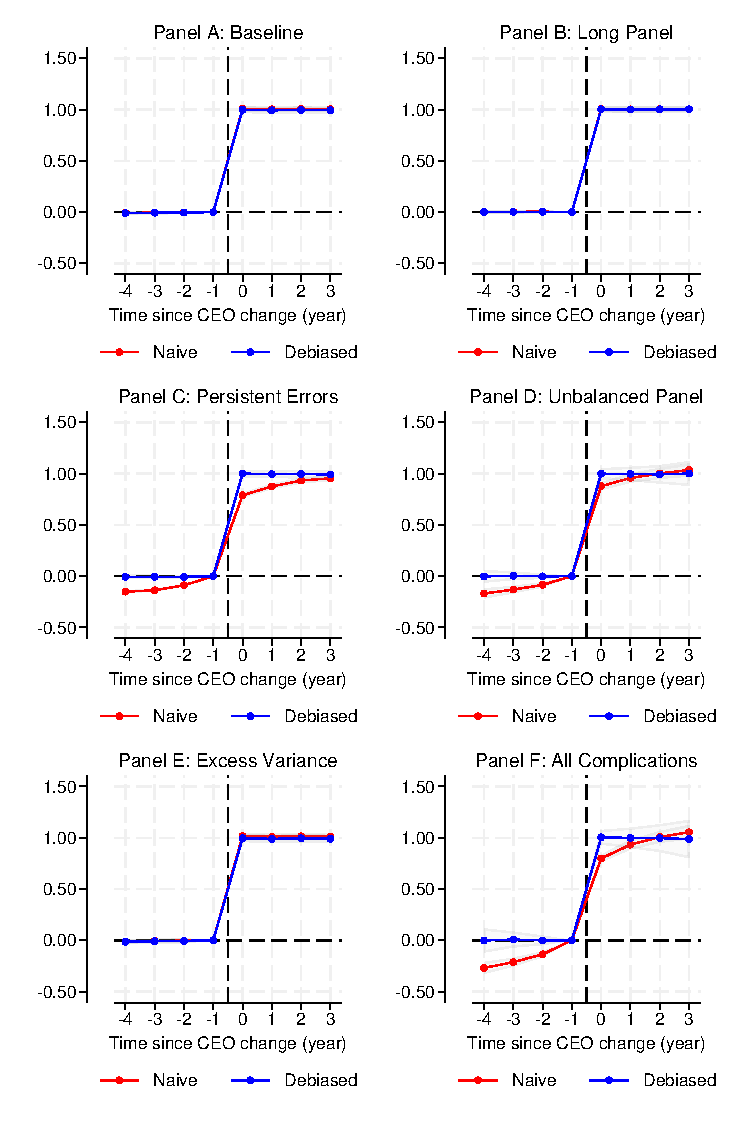
\includegraphics[width=0.95\textwidth]{figure/figuremc.pdf}
\caption{Monte Carlo event studies under six scenarios. Panels: Baseline, Long Panel, Persistent Errors, Unbalanced Panel, Excess Variance, All Complications. Bands are truncated to [-0.75, 1.75] for readability. [[comment: add precise definitions for beta0, beta1, dbeta from the estimator]]}
\label{fig:mc}
\end{figure}

\paragraph{Interpreting Table~\ref{tab:mc_params} and Figure~\ref{fig:mc}.}
Table~\ref{tab:mc_params} reports six Monte Carlo calibrations with different parameters. The baseline is very simple: balanced panels and i.i.d. (uncorrelated) error terms. Across scenarios we focus on three statistics that are widely used in applications: (i) the standard deviation of the change in the manager fixed effect when the firm moves from the first to the second CEO, a key input to variance decompositions; (ii) an event-study slope two full years after the CEO change (the third post year), which captures dynamic adjustment; and (iii) a pre-trend coefficient two years before the change, which should be zero in the data-generating process once the baseline year $t=-1$ is normalized to zero. The debiasing is designed to remove finite-sample noise in all three statistics.

In the baseline, the naive variance is slightly upward biased, while the debiased standard deviation of the manager-effect change recovers exactly 0.10, which is the true value by construction. The post-arrival event-study slope exhibits some sampling noise but nothing systematic. The long-panel scenario (spells of length 20) shows that all biases essentially disappear; this is a small-sample phenomenon in short panels.

With persistent errors ($\rho=0.9$), the naive standard deviation is severely upward biased (about 23\% in our calibration), and spurious pre-trends emerge: before the manager arrives, the naive estimate suggests a negative effect. Because this is a Monte Carlo, we know the true pre-trend is zero; the bias is entirely mechanical. The naive post-arrival slope at $+2$ is below one (about 0.93), consistent with a gradual, biased buildup. Debiasing removes the pre-trend and delivers a post-arrival slope indistinguishable from the true value of 1.00.

The unbalanced-panel scenario (with a 20\% annual hazard of CEO change) compounds persistence and varying spell lengths. We again see a severe upward bias in the variance and evidence of pre-trends in the naive estimates. Debiasing removes these artifacts. Post-arrival dynamics look less gradual than under persistence alone, plausibly because typical spells are shorter in unbalanced panels, leaving less time for any gradual buildup to manifest.

In the excess-variance scenario, the treated group has higher shock variance than controls. Relative to the baseline, this produces more dispersion and a modest upward bias in the naive post-arrival slope; the debiased estimates correct both. Finally, the “all complications” scenario combines short and unbalanced spells, persistent errors, and excess variance. Here all problems are most severe: very large variance bias, pronounced pre-trends before the CEO arrives, and distorted dynamics. Yet the placebo correction handles them jointly: the debiased standard deviation matches 0.10, the post-arrival slope is 1.00, and the pre-trend is 0.00 across all six scenarios. [[note: if you want exact standard errors or scenario-specific percent deviations tabulated, we can add them once the csv outputs are finalized.]]

Figure~\ref{fig:mc} displays event-study slopes for the same six scenarios. The motivation for plotting these is that, with persistent errors and/or unbalanced panels—both common in applications—noise can introduce apparent pre-trends. Researchers routinely check pre-trends, either formally or informally, and may be misled if naive profiles are biased.

Panel A (baseline) shows little bias: differences between naive and debiased lines are barely visible. Panel B (long panel) confirms that bias vanishes with long spells. Panel C (persistent errors) is the key case: the naive profile displays pre-trends and a somewhat sluggish post-arrival adjustment. The intuition is that the naive estimator uses estimated fixed effects that embed noise. With persistence, firms that happen to draw positive shocks over the post period are more likely to be classified as receiving a “good” CEO; by the same logic, their recent past is mechanically below average, generating a spurious pre-trend. The placebo correction strips out precisely this noise component.

Panels D–F illustrate that the problems intensify with unbalanced spells and excess variance, and are most severe when all complications are present. The true event study is the debiased (placebo-corrected) line: it jumps from 0 at $t=0^{-}$ to 1 at $t=0^{+}$ and stays flat thereafter. By contrast, the naive profiles can show strong pre-trends and distorted post dynamics. [[note: confirm which color/style corresponds to naive vs debiased in the final figure legend.]]

We expect to see exactly zero before and exactly one after the arrival of the CEO in TFP units when the true effect is normalized so that a one-unit increase in the fixed effect raises TFP by one. Other outcomes may have different scales, but the logic is the same. With persistence, short spells, or excess variance in treated firms, the naive profiles will typically display pre-trends and inflated post effects; subtracting the placebo series removes these artifacts.

\section{Application: CEO Arrivals and Revenue in Hungarian Firms}

We apply the placebo-controlled debiasing to the universe of Hungarian firms, focusing on CEO arrivals and firm revenue outcomes. The Hungarian data provide an ideal setting because we observe the full population of businesses over three decades, not only large corporations. This scope yields many CEO mobilities across firms, allowing us to study the arrival of new CEOs and the associated within-firm dynamics. We document the data construction, sample restrictions, and additional statistics in our companion paper [[note: add citation to companion paper]]. Here we summarize the minimal features needed for this methodological application and outline the design we will estimate.

We consider all CEO changes between 1992 and 2022 (31 years). We restrict to firms that have ever reached at least 5 employees in their lifetime, to exclude non-employer businesses that rarely change CEOs and would inflate the sample numerically without adding identifying transitions. After this restriction, there are about 60,000 CEO changes [[note: update exact count]]. Many transitions are from the first to the second CEO and from founders to non-founders; these categories are similar but not identical because founders can return later and some firms begin with outsider CEOs. We will include a table with summary statistics for these quantities [[note: add exhibit reference]].

Identification relies on random mobility (strict exogeneity): past and future shocks to outcomes are orthogonal to CEO mobility timing. Because applied work commonly examines pre-trends to assess plausibility, we present event-study profiles grounded in this assumption.

We use firm revenue as the outcome variable for clarity of exposition. We remove industry–year means so that the outcome is measured as a deviation from the sectoral environment.

\subsection*{Estimating CEO Spell Effects}
For each transition from CEO A to CEO B, let the firm have two consecutive spells covering the entire tenures of A and B (not just the event window). We estimate a spell-level CEO effect as the within-spell mean of demeaned revenue. Concretely, let \(r_{it}\) denote firm revenue and let \(\tilde r_{it}=r_{it}-\bar r_{st}\) be revenue demeaned by industry–year \((s,t)\) cells. Let \(\mathbb 1\{\text{spell}=s\}\) indicate the A or B spell. The spell effect is
\begin{equation}
\hat z_{is} = \frac{1}{T_{is}}\sum_{t\in s} \tilde r_{it},\qquad s\in\{A,B\}.
\end{equation}
Define the change in the CEO effect for transition \(i\) by
\begin{equation}
\Delta \hat z_i = \hat z_{iB} - \hat z_{iA}.
\end{equation}
This statistic is the core object in variance decompositions; by theory and by Monte Carlo, its variance is upward biased in short panels and under persistence, which motivates our placebo debiasing.

[[note: if a firm has more than two consecutive spells, we treat adjacent spell pairs as separate transitions; multiple transitions per firm are allowed but clustered at the firm level.]]

\subsection*{Event-Study Specification}
We then study revenue dynamics around CEO arrivals in event time. For each transition with event date \(g\), define dummies for event-time leads/lags relative to \(g\) over the window \([-4,+3]\). We estimate
\begin{equation}
\tilde r_{it} = \alpha_i + \sum_{\ell\in\{-4,-3,-2,0,1,2,3\}} \beta_{\ell}\,\mathbb 1\{t-g=\ell\} + \varepsilon_{it},
\end{equation}
with the baseline period normalized to zero at \(t=-1\). The coefficients \(\beta_{\ell}\) trace out the revenue response before and after CEO arrival. Under random mobility, we expect no pre-trends: \(\beta_{-4},\beta_{-3},\beta_{-2}\approx 0\). Post-arrival dynamics are a question for the data: effects may be immediate or build gradually during the new CEO’s tenure. We will report both naive and placebo-corrected profiles; the latter subtract the corresponding placebo moments computed on matched non-changers with replicated spell designs.

\subsection*{Placebo Construction and Debiasing}
Placebo transitions assign a fake CEO change at the same calendar year as an actual transition to control firms that remain under the same CEO and have long no-change runs covering the event window. We split these control runs into the same pre/post spell lengths as the treated transition and align them in event time. Because the design matrices and weights are the same by construction, and because we assume the error autocovariance (\(\Sigma\)) is the same up to a scalar between treated and placebo groups, the covariance and variance bias components can be “precomputed” in the placebo sample and subtracted from the treated estimates. This delivers debiased variance of \(\Delta \hat z\) and debiased event-study coefficients \(\beta_{\ell}\).

[[note: add the companion paper citation for full data construction and additional outcomes (e.g., investment, materials, labor).]]

Hungary provides an ideal setting for studying CEO effects in the universe of private firms. The country offers complete administrative data coverage for all incorporated businesses, spanning 30 years from the transition economy of the 1990s through EU accession in 2004 to the present. CEO registration is mandatory for every registered firm. The coverage enables us to track CEO careers across firms and construct mobility networks necessary for identification.

Our analysis combines two administrative datasets. The firm registry, maintained by Hungarian corporate courts, contains records on all company representatives — individuals authorized to act on behalf of firms. These records include CEOs and other executives with signatory rights, tracked through a temporal database where each entry reflects representation status over specific time intervals. Updates occur when positions change, personal identifiers are modified, or reporting standards evolve. The registry provides names, addresses, dates of birth (from 2010), and mother's names (from 1999), though numerical identifiers exist only from 2013 onward.

The balance sheet dataset contains annual financial reports for all Hungarian firms with double-entry bookkeeping. The data has information on financial variables and some additional information, such as sector of activity, employment, and ownership (state, domestic, foreign). The two datasets cover 1,063,172 firms over 31 years, yielding 9,627,484 firm-year observations before sample restrictions.

Constructing CEO time series across firms poses some challenges. Before 2013, no numerical identifiers existed, requiring entity resolution based on names, addresses, mother's names, and birthdates. We link records across these dimensions to create unique person identifiers, enabling tracking across firms and over time. Matching quality improves after 1999 (when mother's names reporting begins) and 2010 (when birthdates reporting starts), though the 1990s data achieves reasonable coverage through name and address matching. 

Finding CEOs among all individuals from the data requires heuristics since job titles are inconsistently recorded. When explicit ``managing director'' titles exist, we use them directly. For remaining cases, we assume all representatives are CEOs if three or fewer exist at the firm. When more than three representatives are present, we assign CEO status based on continuity with previously identified CEOs. Time spans between appointments are often unclosed or non-contiguous, requiring imputation based on sequential information, assuming representatives remain active if their tenure includes June 21 of each year.

We apply several restrictions to create a sample suitable for productivity analysis. First, we exclude mining and finance sectors due to specialized accounting frameworks and regulatory environments. Second, we drop firms ever having more than 2 simultaneous CEOs to avoid complex governance structures that complicate identification. Third, we exclude firms with more than 10 CEO changes over the sample period (removing observations for unstable firms) to reduce noise from misclassified transitions. Fourth, we remove all state-owned enterprises, as their objectives and constraints differ from private businesses \citep{orban2019inception, shleifer1994politicians}.

We restrict attention to firms that employ at least 5 workers at some point in the firm lifecycle. This filter removes a substantial portion of observations but eliminates shell companies, tax optimization vehicles, and self-employment arrangements masquerading as corporations. The remaining firms represent genuine businesses with meaningful economic activity where management quality affects performance.

We exclude public firms and joint-stock companies from our analysis. The few companies traded on the Budapest Stock Exchange operate under different governance structures, compensation schemes, and disclosure requirements than private businesses. We also exclude cooperatives and other non-standard corporate forms where multiple managing directors share executive authority, as these organizational structures complicate identification of individual CEO effects.

Firms with multiple CEO changes are handled by splitting their history into adjacent transition pairs. After collapsing firm-CEO spells, intermediate spells are duplicated so that a firm with spells 1/2/3 contributes two transitions, 1$\to$2 and 2$\to$3. Each transition defines a pseudo-firm, indexed by a constructed identifier that groups the true firm with the relevant spell window. Fixed effects are estimated separately for these pseudo-firms, so outcomes around different transitions are allowed to have distinct firm intercepts. These pseudo-firms are not treated as independent statistical units. We retain the original firm identifier and cluster standard errors by the true firm. 



\begin{comment}
Jó lenne a mintára csinálni, és nem a populációra
Kellene néhány céges jellemző (emp, TFP) az A panelbe
Kellene az átlag (átlagosan hány CEOja van egy cégnek, és egy CEO átlagosan mennyit van a cégnél)
\end{comment}

Appendix Table \ref{tab:sample} presents the number of firms in our sample relative to the total number of firms in the data for several year along the time series. The number of Hungarian firms increases abruptly during the nineties and also in the first 15 years of 2000s, albeit at a smaller pace.  The result of dropping the small firms results in using about one quarter of all firms. In the first year of study (1992) we have 26 thousand firms which increases to 115 thousand towards the end of the period. Overall, we have over one million firms and almost 10 million firm-years in the sample. The table also shows the number of CEOs each year, which presents a similar pattern; in 1992 we observe 32 thousand CEOs and in 2022 122 thousand. The total number of distinct CEOs is 340 thousand. Appendix Table \ref{tab:industry_stats} shows the industrial distribution of firms and CEOs. The largest sectors are Wholesale-Retail, Telecom and Business Services and Nontradable Services. 

Table \ref{tab:CEO_desc} shows the proportion of firms (and firm-years) by the number of CEOs observed in the firm during the period of observation. Not surprisingly, a majority of firms have only one CEO: 63\% of firms and 80\% of firm-years belong to this category. One quarter of firms had two CEOs while 13\% at least three CEOs. This latter category comprises only 3\% of firm-years. CEO spell lengths follow an exponential distribution with a 20 percent annual hazard rate, implying typical tenures of 3-7 years.


%%%%%%%%%%%%%%%%%
\section{Results}
%%%%%%%%%%%%%%%%% 

We present event studies examining revenue dynamics around CEO transitions. Figure \ref{fig:application} displays four key moments around CEO arrivals: variance of revenue changes (Panel A), the share of revenue variance explained by CEO transitions (Panel B), covariance of revenue with CEO effects (Panel C), and regression coefficients (Panel D). Each panel compares naive OLS estimates (red) with placebo-corrected debiased estimates (blue).

\begin{figure}[htbp]
\centering
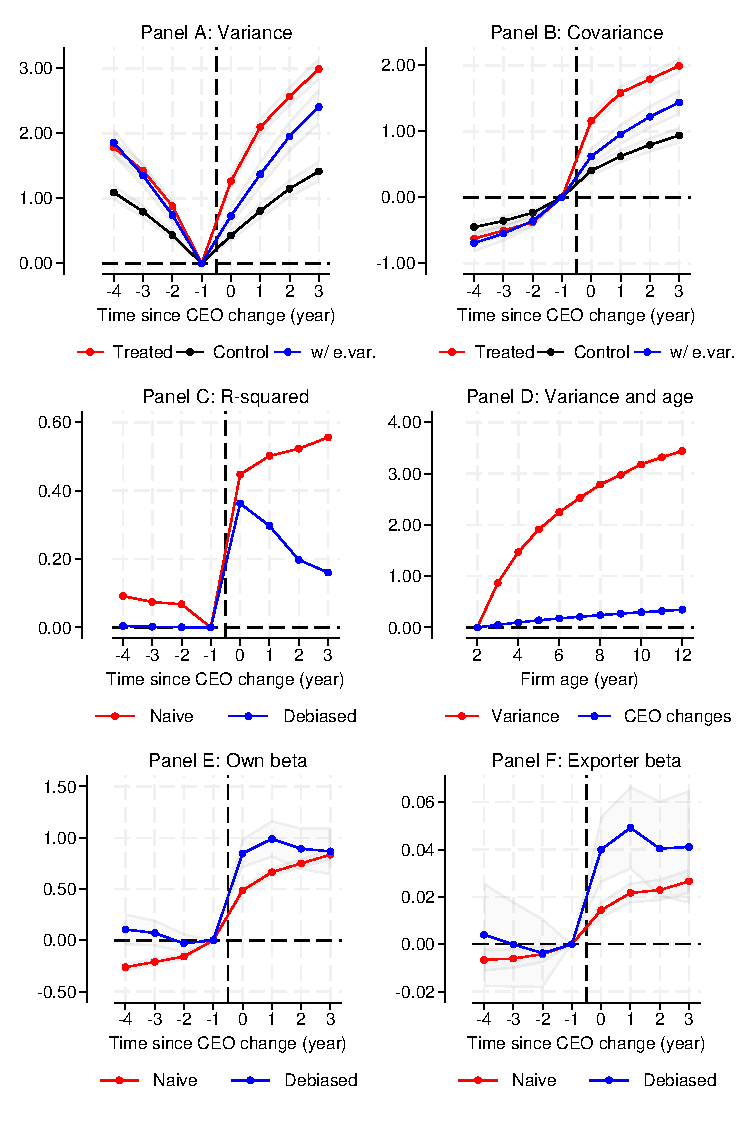
\includegraphics[width=0.95\textwidth]{figure/application.pdf}
\caption{Revenue Dynamics Around CEO Transitions in Hungarian Firms}
\label{fig:application}
\begin{minipage}{0.95\textwidth}
\footnotesize
Notes: Event studies of log revenue around CEO transitions. All panels normalize to year $t=-1$ (one year before CEO arrival). Panel A shows the variance of revenue changes from baseline. Panel B displays the fraction of revenue variance explained by CEO fixed effects (R-squared). Panel C plots the covariance of revenue change with the change in CEO fixed effect. Panel D shows regression coefficients from projecting revenue on CEO effects. Red lines show naive OLS estimates; blue lines show placebo-corrected debiased estimates. Shaded regions indicate 95\% confidence intervals. The placebo group consists of matched non-changing firms from the same birth cohort and sector, assigned pseudo CEO transitions at the same calendar year as treated firms. Event window spans $[-4, +3]$ years around CEO arrival.
\end{minipage}
\end{figure}

\paragraph{Variance Dynamics (Panel A).} The variance of revenue changes increases as we move away from the baseline year $t=-1$ because firms accumulate shocks over time. The naive estimate (red) shows continuous growth in variance. After debiasing (blue), we see that much of this variance is mechanical noise rather than CEO effects. The debiased estimate reveals a discrete increase in variance after the new CEO arrives, indicating that CEO transitions genuinely increase outcome dispersion. We also observe slightly elevated variance before the transition, suggesting that firms experiencing CEO changes may be somewhat more volatile than matched controls even before the change. This hints at a mild violation of strict exogeneity, though the effect is small relative to the post-transition jump.

\paragraph{Variance Decomposition (Panel B).} Panel B translates the variance estimates into an R-squared: the fraction of revenue variance explained by CEO fixed effects. This should be zero before the CEO arrives. The debiased estimate confirms this: there is no explanatory power of future CEO identity on past revenue. After the CEO arrives, the naive estimate suggests CEO effects explain nearly 60\% of revenue variance. The debiased estimate shows this is severely upward biased. Three years after arrival, approximately 28\% of revenue variation stems from CEO effects---substantial, but only half the naive estimate. This decomposition demonstrates that ignoring small-sample bias dramatically overstates the role of CEOs in firm performance.

\paragraph{Covariance Dynamics (Panel C).} The covariance of revenue change with the change in CEO fixed effect provides a direct test for pre-trends. The naive estimate (red) displays strong spurious pre-trends: past revenue appears to predict future CEO quality. Under strict exogeneity, past revenue should be uncorrelated with future CEO effects, so this is entirely bias. The debiased estimate (blue) removes these pre-trends. Before the CEO arrives, covariance fluctuates around zero with no significant pattern. After arrival, covariance becomes positive, consistent with better CEOs generating higher revenue.

\paragraph{Regression Coefficients (Panel D).} Panel D rescales the covariance and variance into regression slopes, measuring revenue response per unit of CEO quality. This is a nonlinear transformation (ratio of covariance to variance), so standard errors are larger via the delta method. The naive estimate shows pronounced pre-trends and a gradual post-arrival buildup. The debiased estimate eliminates the pre-trend and reveals immediate, persistent effects. The CEO effect on revenue is approximately one-for-one (by construction of the CEO fixed effect normalization) and appears in year zero, remaining stable through year three. This suggests CEO impacts are immediate rather than gradual, contradicting the sluggish adjustment implied by naive estimates.

%elég 3 tizedesjegy, nem vagyunk mink atom fizikusok
%a nobs nem jó, mert három különböző kell a három sorba

\paragraph{CEO Transitions and Productivity Change.} Table \ref{tab:placeholder} shows the average effect of CEO transition on productivity as estimated by the naive OLS regression, the placebo effect and the corrected regression estimate.\footnote{The naive and the pseudo outcome regression are estimated on the treated and placebo samples, respectively. The controls are the not-yet-treated firm years. The corrected regressions are estimated on the merged samples and we use the two-way treatment method discussed in Section \ref{sec:est}.} To start with the effect on the whole sample, TFP increases by 0.5\% around the CEO change. The placebo regression produces precisely measured zeros.\footnote{This is reasonable because here we do not have a reason to believe the estimated effect by simple OLS regression is biased as we do not select on unobservables correlated with productivity.} That is, even without a CEO change, TFP changes somewhat. The placebo controlled estimate equals 0.3\%.

As most of our firms are family-owned, we look into an interesting CEO transition: when founders relinquish control. For comparison, we also run a separate regression on other CEO changes. When founders are the departing CEO, the estimated effect is 1\%. For the other CEO changes we do not find any change in TFP. This is also a test of our method: when similar CEOs replace each other, the effect is zero, at least on average. On the contrary, when we measure the TFP change between two distinctly different CEOs, we do find an economically and statistically significant effect.\footnote{The reason for a positive effect of founder replacement may be the timing of the change. Founders usually give up their central role in the firm when they find they no longer have enough energy to run the firm.} 



Finally, we analyze perhaps the most interesting question: how the productivity reacts to the arrival of a better or worse CEO than the incumbent? For this, we split the sample into two types of CEO transitions: when the incoming CEO has a higher or lower quality (as measured by the associated fixed effect) than the incumbent CEO. We also split the placebo sample into firms which experience an increase/decline of their TFP around the pseudo CEO change. The estimated coefficients are presented in the last two columns of Table \ref{tab:placeholder} and demonstrate the importance of CEOs and also show how the placebo correction works. Better CEOs than the incumbent increase TFP by 6\% while worse CEOs decrease it by 5\%. This large effect, however, is upward biased, as the placebo regressions demonstrate. The pseudo CEO change also produces a sizable effect of $\pm$2.5\%. Thus, the corrected effect is much smaller: better CEOs increase TFP by 2.7\% while worse CEOs decrease it by 1.8\%. Thus, the difference between a good and a bad CEO is 4.5\%. 

Figure \ref{fig:event_study_main} visualizes the evolution of TFP around the CEO change for four samples: all changes, when the incumbent is the founder of the firm, all other incumbents, and for the period of mature market economy (2004 -- 2022).\footnote{The latter sample is used to make our results more comparable to mature market economies. In the 1990s the economy was changing rapidly as it underwent rapid economic liberalization, transition to market economy, foreign direct investment inflows and large scale privatization. We conduct this robustness check by restricting the sample to post-2004 data following Hungary's EU accession.} On each figure we present the event time regression estimates for the whole sample (black line) and for better and worse CEO replacements (blue and red lines). The estimations leave little pre-trend and we find large swings in TFP. If the incoming CEO is better than the incumbent, TFP increases by 3 -- 4\% while worse CEOs decrease it by about 2\%. New CEOs have an effect immediately on the firm and this proves to be quite stable, as the estimated coefficients do not change much.  



\paragraph{Differential Effects on Inputs.} Figure \ref{fig:event_study_input} presents event studies examining how CEO transitions affect different firm inputs.

Good CEOs have immediate and substantial effects on operational inputs. Material costs increase by 30\% and the wage bill by 13 percent (all effects highly significant). Firms under bad managers experience the opposite: a decline in material and employment costs by about 20\%. These effects appear immediately in the year of CEO transition and persist throughout the post-period, consistent with new CEOs quickly adjusting operational scale.

In contrast, strategic variables show different patterns. Fixed assets exhibit a gradual change under good CEOs and little or no change under bad CEOs. The proportion of firms with intangible assets does not change at all around the CEO transition.

\paragraph{Contribution of CEOs to Firm Productivity.} To assess how important CEOs are for firm performance, we conduct the variance decomposition. As we describe at the end of Section \ref{sec:est}, we face two challenges. The variance is biased and it also depends on firm age. The outcome of our method is presented in Figure \ref{fig:variance_decomp} for TFP in the top row and log revenue in the bottom row. The blue line shows the within-firm change in variance relative to the second year after firm foundation. The blue line on panels A and C show the evolution of this variance around the CEO transition. Before the CEO transition, the variance grows continuously. The transition increases the variance abruptly; in later years it stays relatively stable for TFP and continues growing for revenue. Part of this growth, however, is due to limited mobility bias, and part arises mechanically: as time passes, the chance of receiving shocks increases. To control for these biases, we estimate the same variance on the pseudo transition sample. As the red line shows, this also increases in time. Panels B and D of the figure show the evolution of the estimated variance in the two samples by firm age. 

Our estimate of the contribution of CEO change to the total variance of TFP is the difference between the two estimates, and we quantify it in Appendix Table \ref{tab:var_share}. The table presents the total variance, the unadjusted contribution of CEO change and the adjusted contribution. We analyze only one CEO change, and the contribution depends on the length of the period measured (the longer the period, the more the variance increases for reasons unrelated to CEO change). In the first 10 years of existence, the uncorrelated share of CEO change in the variance is 62\%. Our correction decreases this number to 29\%.




%%%%%%%%%%%%%%%%%%%%
\section{Conclusion}
%%%%%%%%%%%%%%%%%%%%

This paper estimates the contribution of CEOs to firm productivity by exploiting a unique administrative dataset covering the entire population of Hungarian private firms and their CEOs from 1992 to 2022. The novelty of the data lies in its unprecedented scope and completeness, allowing the study of CEO effects not only in large firms but crucially in small and medium-sized enterprises that dominate every economy. The combination of the dataset with a theoretically grounded model that distinguishes owner-controlled capital decisions from CEO-controlled operational inputs allows for a more precise attribution of productivity effects. 

The paper develops a new placebo-controlled event study design that overcomes limited mobility bias, which contaminates studies using two fixed effects.  By creating matched placebo CEO transitions in firms without actual leadership changes, the method effectively separates true CEO skill effects on productivity from mechanical noise. Empirically, the findings reveal that the true causal effect of CEO quality on firm productivity is economically meaningful but notably smaller than raw correlations suggest, explaining about 7–8 percent of productivity variation. 

An alternative way to deal with the noise problem is to use observable manager characteristics as measures of skill. Observable characteristics such as education and work experience \citep{DePirro2025}, foreign name as a proxy for international exposure \citep{Koren2023expat}, and the selectiveness of entry cohorts \citep{koren2024managers} offer more reliable, though narrower, measures of specific dimensions of managerial quality. These observables capture only partial aspects of CEO ability but avoid the mechanical noise that contaminates fixed effects estimates.

\clearpage
\bibliographystyle{apalike}
\bibliography{lib/references}

\clearpage
\appendix
\section{Online Appendix: Additional Tables and Figures}
\renewcommand{\thefigure}{A\arabic{figure}}
\renewcommand{\thetable}{A\arabic{table}}
\setcounter{figure}{0}
\setcounter{table}{0}




%Benne maradhat a populáció, de kellene a minta is. Esetleg kidobhatjuk a firms oszlopot, és készítsük el a táblát a populációra és a mi mintánkra (Population: firm-year CEO, Sample: firm-year CEO, Surplus Share)


%\begin{table}[htbp]\centering
\def\sym#1{\ifmmode^{#1}\else\(^{#1}\)\fi}
\caption{Surplus Function Estimation Results}
\begin{tabular}{l*{6}{c}}
\toprule
                    &\multicolumn{1}{c}{(1)}&\multicolumn{1}{c}{(2)}&\multicolumn{1}{c}{(3)}&\multicolumn{1}{c}{(4)}&\multicolumn{1}{c}{(5)}&\multicolumn{1}{c}{(6)}\\
                    &\multicolumn{1}{c}{Revenue}&\multicolumn{1}{c}{EBITDA}&\multicolumn{1}{c}{Wagebill}&\multicolumn{1}{c}{Materials}&\multicolumn{1}{c}{Revenue}&\multicolumn{1}{c}{Revenue}\\
\midrule
Fixed assets (log)  &       0.323\sym{***}&       0.325\sym{***}&       0.287\sym{***}&       0.375\sym{***}&       0.290\sym{***}&       0.295\sym{***}\\
                    &     (0.001)         &     (0.001)         &     (0.001)         &     (0.002)         &     (0.001)         &     (0.004)         \\
\addlinespace
Has intangible assets&       0.268\sym{***}&       0.163\sym{***}&       0.267\sym{***}&       0.317\sym{***}&       0.205\sym{***}&       0.255\sym{***}\\
                    &     (0.003)         &     (0.003)         &     (0.003)         &     (0.004)         &     (0.003)         &     (0.010)         \\
\addlinespace
Founding owner      &      -0.079\sym{***}&      -0.051\sym{***}&      -0.017\sym{***}&      -0.099\sym{***}&      -0.010\sym{***}&      -0.015\sym{*}  \\
                    &     (0.005)         &     (0.005)         &     (0.005)         &     (0.006)         &     (0.003)         &     (0.008)         \\
\addlinespace
Non-founding owner  &      -0.001         &      -0.000         &      -0.003         &      -0.006         &      -0.011\sym{***}&      -0.017\sym{*}  \\
                    &     (0.007)         &     (0.006)         &     (0.007)         &     (0.009)         &     (0.004)         &     (0.009)         \\
\addlinespace
Foreign owned       &       0.025\sym{**} &       0.018         &       0.064\sym{***}&       0.010         &       0.022\sym{*}  &       0.033         \\
                    &     (0.012)         &     (0.012)         &     (0.012)         &     (0.015)         &     (0.011)         &     (0.025)         \\
\addlinespace
State owned         &       0.148\sym{***}&       0.047\sym{*}  &       0.448\sym{***}&       0.146\sym{***}&       0.062\sym{**} &       0.050         \\
                    &     (0.029)         &     (0.028)         &     (0.029)         &     (0.032)         &     (0.026)         &     (0.059)         \\
\midrule
Observations        &     3004184         &     2326192         &     2949024         &     3059662         &     2967233         &      374084         \\
\bottomrule
\multicolumn{7}{l}{\footnotesize Standard errors in parentheses}\\
\multicolumn{7}{l}{\footnotesize All models include firm fixed effects, industry-year fixed effects, and a step function for firm age.}\\
\multicolumn{7}{l}{\footnotesize Outcome variables are log-transformed. Models (5) and (6) include quadratic controls for CEO age and tenure.}\\
\multicolumn{7}{l}{\footnotesize Model (6) restricts to largest connected component of CEO-firm network.}\\
\multicolumn{7}{l}{\footnotesize \sym{*} \(p<0.10\), \sym{**} \(p<0.05\), \sym{***} \(p<0.01\)}\\
\end{tabular}
\end{table}




\end{document}








\appendix
\section{Online Appendix: Additional Tables and Figures}
\renewcommand{\thefigure}{A\arabic{figure}}
\renewcommand{\thetable}{A\arabic{table}}
\setcounter{figure}{0}
\setcounter{table}{0}

\subsection{Production Manager Autonomy in Family Firms}

%\begin{table}[htbp]\centering
\def\sym#1{\ifmmode^{#1}\else\(^{#1}\)\fi}
\caption{Plant Manager Autonomy in Family-Controlled Firms}
\begin{tabular}{l*{5}{c}}
\toprule
                    &\multicolumn{1}{c}{(1)}&\multicolumn{1}{c}{(2)}&\multicolumn{1}{c}{(3)}&\multicolumn{1}{c}{(4)}&\multicolumn{1}{c}{(5)}\\
                    &\multicolumn{1}{c}{Investment}&\multicolumn{1}{c}{Investment}&\multicolumn{1}{c}{Marketing}&\multicolumn{1}{c}{Product}&\multicolumn{1}{c}{Hiring}\\
\midrule
Family ownership    &      -0.369\sym{**} &      -0.200\sym{**} &      -0.344\sym{**} &      -0.299\sym{**} &       0.086         \\
                    &     (0.161)         &     (0.100)         &     (0.153)         &     (0.151)         &     (0.068)         \\
\midrule
Observations        &       2,915         &       2,379         &       3,133         &       3,114         &       3,138         \\
Country FE          &         Yes         &         Yes         &         Yes         &         Yes         &         Yes         \\
Industry FE         &         Yes         &         Yes         &         Yes         &         Yes         &         Yes         \\
\bottomrule
\multicolumn{6}{l}{\footnotesize Standard errors in parentheses}\\
\multicolumn{6}{l}{\footnotesize Data source: Bloom, Sadun, and Van Reenen (2012). Sample restricted to private (non-publicly traded) firms.}\\
\multicolumn{6}{l}{\footnotesize Investment autonomy measured as maximum capital investment plant manager can approve (USD).}\\
\multicolumn{6}{l}{\footnotesize Other autonomy dimensions are binary indicators for full autonomy (score = 5 on 1-5 scale).}\\
\multicolumn{6}{l}{\footnotesize PPML = Poisson Pseudo-Maximum Likelihood. Standard errors clustered at firm level.}\\
\multicolumn{6}{l}{\footnotesize All specifications include country and 2-digit SIC industry fixed effects.}\\
\multicolumn{6}{l}{\footnotesize \sym{*} \(p<0.10\), \sym{**} \(p<0.05\), \sym{***} \(p<0.01\)}\\
\end{tabular}
\end{table}


\subsection{Industry Breakdown}

%

%\begin{table}[htbp]\centering
\def\sym#1{\ifmmode^{#1}\else\(^{#1}\)\fi}
\caption{The revenue function by sector}
\begin{tabular}{l*{6}{c}}
\hline\hline
                    &\multicolumn{1}{c}{(1)}&\multicolumn{1}{c}{(2)}&\multicolumn{1}{c}{(3)}&\multicolumn{1}{c}{(4)}&\multicolumn{1}{c}{(5)}&\multicolumn{1}{c}{(6)}\\
                    &\multicolumn{1}{c}{Agriculture}&\multicolumn{1}{c}{Manufacturing}&\multicolumn{1}{c}{Wholesale, Retail, Transportation}&\multicolumn{1}{c}{Telecom and Business Services}&\multicolumn{1}{c}{Construction}&\multicolumn{1}{c}{Nontradable services}\\
\hline
Tangible and intangible assets (log)&       0.320\sym{***}&       0.296\sym{***}&       0.257\sym{***}&       0.237\sym{***}&       0.281\sym{***}&       0.207\sym{***}\\
                    &     (0.006)         &     (0.003)         &     (0.002)         &     (0.002)         &     (0.002)         &     (0.002)         \\
[1em]
Intangible assets share&       0.071         &       0.011         &      -0.006         &      -0.057\sym{***}&       0.029         &      -0.020         \\
                    &     (0.059)         &     (0.025)         &     (0.014)         &     (0.013)         &     (0.030)         &     (0.015)         \\
[1em]
Foreign owned       &      -0.070\sym{*}  &       0.046\sym{*}  &       0.008         &       0.082\sym{***}&      -0.055         &      -0.013         \\
                    &     (0.042)         &     (0.024)         &     (0.015)         &     (0.022)         &     (0.041)         &     (0.015)         \\
\hline
Observations        &      208269         &      748880         &     1893882         &     1224209         &      630073         &     1708957         \\
\hline\hline
\multicolumn{7}{l}{\footnotesize Controls: firm-CEO-spell fixed effects; industry-year fixed effects.}\\
\end{tabular}
\end{table}



\subsection{Manager Skill Distributions}

\begin{figure}[htbp]
\centering
\begin{minipage}{0.48\textwidth}
\centering
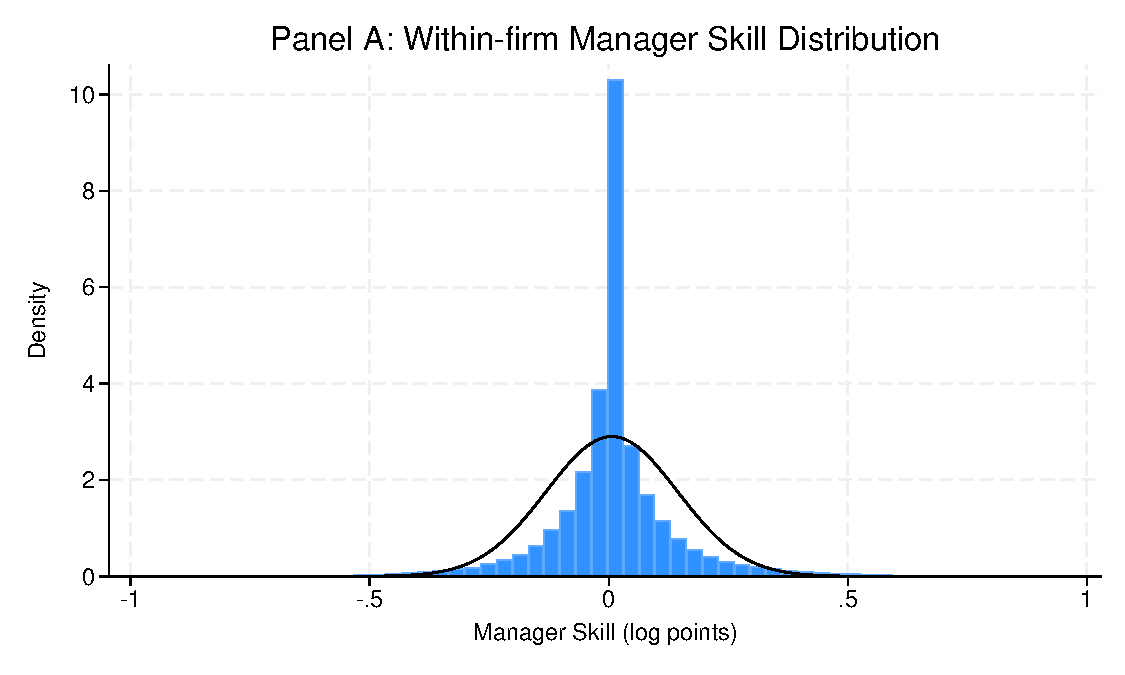
\includegraphics[width=\textwidth]{figure/manager_skill_within.pdf}
\end{minipage}
\hfill
\begin{minipage}{0.48\textwidth}
\centering
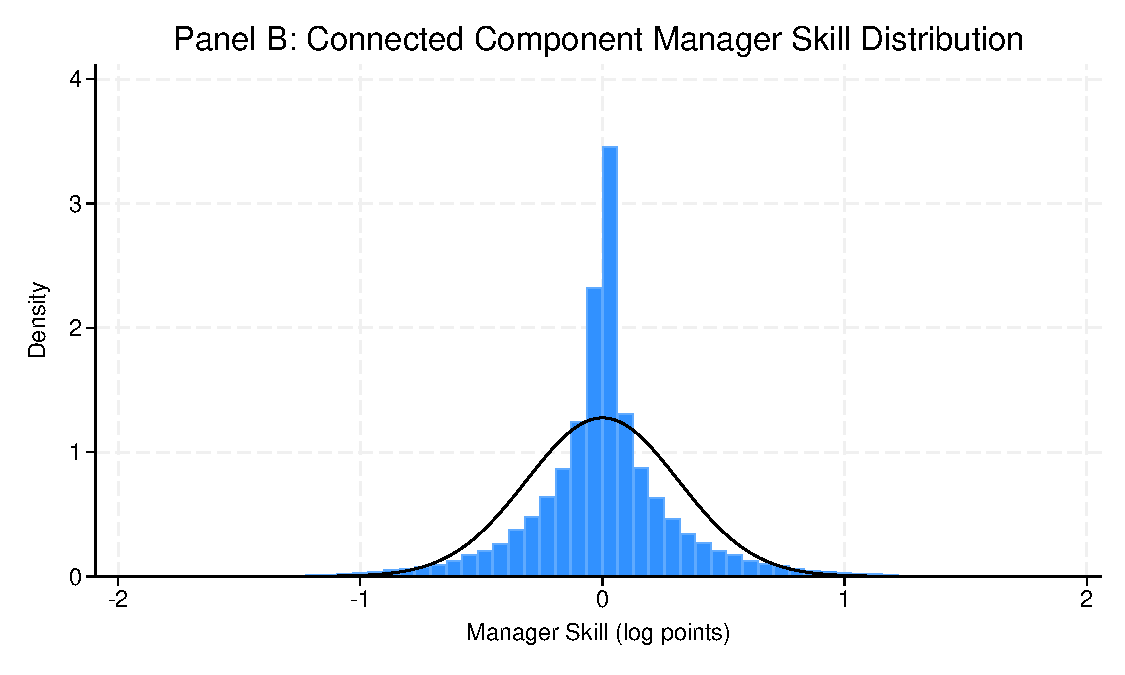
\includegraphics[width=\textwidth]{figure/manager_skill_connected.pdf}
\end{minipage}
\caption{Manager Skill Distributions}
\label{fig:manager_skills_appendix}
\footnotesize
Notes: Panel A shows the distribution of within-firm manager skill variation for firms with multiple CEOs. Panel B shows the distribution of manager skills in the largest connected component of managers. Both distributions show manager skills in log points after normalization and scaling.
\end{figure}


% Additional tables and figures to be inserted here as needed

\subsection{Variance-Based Evidence for CEO Heterogeneity}



Figure \ref{fig:variance_event_study} presents complementary evidence using the variance of log TFP around CEO transitions. Under our framework, if CEO changes introduce real heterogeneity in managerial quality, the cross-sectional variance of outcomes should increase at the transition point—some firms get better CEOs, others get worse ones. In contrast, pure noise or firm-specific trends would not systematically alter variance.

The variance analysis shows that actual CEO transitions are associated with increased dispersion in outcomes, while placebo transitions show no such effect. This provides model-free evidence that CEO transitions introduce real heterogeneity in firm performance, supporting our identification strategy.


\subsection{Treatment Effects on Owner vs Manager Variables}

{
\def\sym#1{\ifmmode^{#1}\else\(^{#1}\)\fi}
\begin{tabular}{l*{3}{c}}
\hline\hline
                    &\multicolumn{1}{c}{(1)}&\multicolumn{1}{c}{(2)}&\multicolumn{1}{c}{(3)}\\
                    &\multicolumn{1}{c}{Fixed assets (log)}&\multicolumn{1}{c}{Has intangible assets}&\multicolumn{1}{c}{Foreign owned}\\
\hline
Better CEO          &       0.054         &       0.056\sym{***}&       0.051\sym{***}\\
                    &     (0.078)         &     (0.020)         &     (0.013)         \\
\hline
Observations        &       81272         &       81272         &       81272         \\
\hline\hline
\end{tabular}
}


{
\def\sym#1{\ifmmode^{#1}\else\(^{#1}\)\fi}
\begin{tabular}{l*{2}{c}}
\hline\hline
                    &\multicolumn{1}{c}{(1)}&\multicolumn{1}{c}{(2)}\\
                    &\multicolumn{1}{c}{Wagebill (log)}&\multicolumn{1}{c}{Materials (log)}\\
\hline
Better CEO          &       0.055\sym{***}&       0.127\sym{***}\\
                    &     (0.013)         &     (0.013)         \\
\hline
Observations        &     1089713         &     1089713         \\
\hline\hline
\end{tabular}
}

